% Chapter 1

\chapter{Implementation} % Main chapter title

\label{Chapter3} % For referencing the chapter elsewhere, use \ref{Chapter1} 

\lhead{Chapter 3. \emph{Implementation}} % This is for the header on each page - perhaps a shortened title

%----------------------------------------------------------------------------------------
\noindent In this chapter we highlight our design choices and implementation details of the proposed solution.

\section{Domain-specific Language}


%----------------------------------------------------------------------------------------

\noindent After the selection of the suitable declarative approach for building our prototype we can start with the creation of the domain-specific language that shall allow the specification of the provisioning and deployment plans. The motivation here is that there are languages available that allow the specification of workflows (plans), but they are too generic. We want our language to be specific to the deployment and provisioning domain. Thus, it is important to identify language constructs that are relevant to this domain and also to the specification of the deployment plan execution logic. From the other side, to release engineers from learning new notations, our DSL shall be compliant to the main workflow definition languages, such as PetriNets\footnote{ Petri Nets World, $  $http://www.informatik.uni-hamburg.de/TGI/PetriNets/}, BPMN\footnote{ BPMN 2.0 standard, $  $http://www.omg.org/spec/BPMN/2.0/} or WS-BPEL\footnote{ WS-BPEL 2.0 standard, $  $http://docs.oasis-open.org/wsbpel/2.0/OS/wsbpel-v2.0-OS.html}, or UML Activity Diagrams\footnote{ UML 2.0 standard, $  $http://www.uml.org/\#UML2.0}. For the sake of clarity we shall state that BPMN and UML are more related to the workflows design phase, while WS-BPEL - to the workflows implementation phase, and PetriNets may be used for both. We are interested in the design and implementation phases, so we analyze them together.

\noindent 

\noindent A short overview of these languages:

\begin{enumerate}
\item  PetriNets is a graphical and mathematical modeling tool that can be used in many different systems \cite{murata1989petri}: concurrent, asynchronous, nondeterministic and distributed. PetriNets may be used by theoreticians to model systems and analyze them as well as by practitioners in real-world scenarios to execute some processes. PetriNet itself is a directed graph with two kinds of nodes -- places (circles) and transitions (rectangles), and arcs that may lead either from place to transition or from the transition to a place. Places are holders of tokens and transitions are consumers and producers of tokens. Tokens are used to enable the execution of events (transitions). By simulating a movement of tokens from one place to another, the execution of a process/workflow may be analyzed.

\item  BPMN stands for Business Process Model and Notation and is a standard to represent processes in virtually any kind of organization \cite{chinosi2012bpmn}. Its primary goal is to provide a notation for the business processes that can be clearly understood by the business and technical users at the same time. A business process is represented in a Business Process Diagram which consists of Flow Objects (Events, Activities, Gateways) which determine behavior of the business process; Connecting Objects (Sequence Flow, Message Flow, Associations) to connect objects to each other; Swimlanes (Pools and Lanes) for grouping a set of elements; Artifacts (Data Object, Group, Annotation) for providing additional information. BPMN 2.0 provides the ability to model new sets of processes such as Orchestrations, Choreographies and Collaborations and puts more emphasis on the importance of Data.

\item  WS-BPEL is a language for the specification of the executable and abstract business processes, based exclusively on Web Services. It defines the model and grammar to describe the behavior of a business processes. Executable business processes model actual behavior of a given participant of the process, while Abstract business processes serve a descriptive role and may be used in more than one use case. The specification consists of partnerLinks -- to defined different parties involved in the business process, variables -- to represent data, faultHandlers -- activities that must be performed in case of errors in the process and the process itself. The process in turn consists of different activities: some of them are directly linked to web services like receive, reply, invoke; others define the structure and ordering of the other activities in the process - like sequence, flow, scope, wait, forEach, while and more.

\item  UML Activity Diagram is part of the UML (a graphical notation for modeling object-oriented systems) and shows activities and actions to describe workflows   \cite{JOT:issue_2003_07/column3}. The diagram itself consists of nodes (action, structured, control and object nodes) and edges (control and object flow edges). In addition to that, different kinds of events may be added. 
\end{enumerate}

\noindent 

\noindent It is important to mention here that pure PetriNets cannot be compared with BPMN or UML Activity Diagrams as they do not have any way to represent data objects, so when we talk about PetriNets we actually refer to their variant called Colored PetriNets \cite{jensen1991coloured} in which it is possible to represent any kind of data, time constraints and more.

%----------------------------------------------------------------------------------------
\subsection{Selection of the Language Constructs and Language Representation}

\noindent All of these languages have similar expressive power \cite{geambacsu2012bpmn, storrle2004semantics, hinz2005transforming}, so it is possible to describe most workflows in any of them, although the effort to do that will differ from one language to another. By the similar expressive power we mean that they all share (under different names, of course) such constructs as actions, control and data nodes, control and data flows, and different kinds of events. Control nodes and flows are used to determine the ordering of actions (for instance, concurrent execution of tasks, which is essential for the deployment of large-scale cloud applications), data nodes and flows are used to pass objects from one action to another, and actions themselves -- for the actual execution of the workflow. In addition, events may be used to handle errors or interactions with users, or communication between different workflows. 

\noindent 

\noindent In practice, as stated in \cite{zur2008much}, some constructs of these languages may not be needed: ``... the complexity of BPMN in practice differs considerably from its theoretical complexity. This, in turn, suggests that future research should take this distinction into account when considering BPMN's expressive power, complexity or other features or characteristics''. That is why from the list of constructs that we just discussed, we have to choose which of them are relevant to the deployment activities and are useful to define the proper ordering of tasks in the deployment plan.

\noindent 

\noindent A small set of language constructs could also be justified by the analysis of the deployment approaches that usually have the same set of common tasks such as download, install, configure, start, and stop. The need for events, error handlers, and some types of control nodes is quite questionable in the context of the deployment process:

\noindent 

\begin{enumerate}
\item  as long as the application topology model is ready (declarative approaches) or deployment plan is created (imperative approaches), no interaction with the user is usually expected during the execution of the deployment plan, so receive events are not needed; timer events could be useful but in most cases they may be eliminated by the proper synchronization of different tasks. And even if they are really needed - users of our DSL would be able to represent them as normal tasks (probably with a specific name ``timer'') without the need to add more constructs to the DSL itself.

\item  as for error handling events, we argue that errors during the deployment plan executions happen most often because of improper design of the application topology model, so it is better to fix the model and rerun the deployment, rather then handle errors on the fly. In case error happenned because of another reason (maybe downtime of the cloud provider service), error handling events would still be useless, most probably, because error of one component could lead to the missconfiguration of a bunch of other components. Moreover, even if application operators had an opportunity to handle errors on the fly, the installation of other components that depend on the failed one could time out or make the whole process infinitevily long, if more than one component failed. We believe the deployment process, or at least parts of it, shall have transactional nature -- either succeed or fail. In addition, handling error scenarios is out of scope of this work.  

\item  as for control nodes, tasks such as fork and join are definitely useful for concurrent execution, while it is hard to justify the need for decision and merge nodes because deployment process is a well-planned activity and there shall not be place for any ambiguities.

\item  the need for recurring actions (for and while loops) is also questionable: during the deployment developers may think of recurring actions when it is required to provision a bunch of identical virtual machines, but in that case running such installation in a loop would not make sense because it would be sequential execution and would take a lot of time, so in such case parallel execution is the way to go.

\item  one more observation that was made during the analysis of the deployment tools and approaches - we do not need asynchronous invocation of actions as one task shall not be started before the previous one completes (unless tasks are independent - then we can run them in parallel, but still in a synchronous mode). For instance, installation of the web server can not be started before the virtual machine has been provisioned, so there is no reason to invoke provisioning task asynchronously and continue the deployment process while provisioning task is running.
\end{enumerate}

\noindent 

\noindent Following this discussion, our initial language constructs set may consist of the following elements: 

\begin{enumerate}
\item  control flow to trigger tasks in the deployment plan

\item  data flow to exchange objects between tasks

\item  a task/action node that would represent all kinds of deployment operations

\item  object node to save some variables

\item  start and stop nodes

\item  fork and join nodes to parallelize and synchronize execution of multiple independent tasks

\item  grouping node to execute a set of identical tasks in parallel can be very useful in large-scale applications to keep the deployment plan readable
\end{enumerate}

\noindent Every workflow language mentioned previously contains such set of constructs, so any of them could be used to create our DSL. Nevertheless, these languages were not designed for the same purpose. BPMN is better known in the business world. BPEL, to some extent, is an executable version of the BPMN \cite{ouvans2006bpmn}, so it is mostly known to developers of the business process applications. In addition, BPEL relies exclusively on Web Services as we stated before, while deployment process has little to do with Web Services (except maybe establishing connections to the cloud provider). Finally, PetriNets and UML Activity diagrams are both very well-known modeling tools and are used in many different domains, but we believe that UML Activity Diagrams are easier to read or to learn, and more familiar to developers what is quite important in the context of deployment tools.

\noindent 

\noindent Based on such observations and assumptions we decided that DSL for the deployment and provisioning shall be similar/compliant to UML Activity Diagrams.

%----------------------------------------------------------------------------------------
\subsection{Metamodel of the Provisioning and Deployment DSL}

\noindent To formalize our DSL we refer to the software development paradigm called model-driven engineering (MDE) \cite{kent2002model}. In MDE, models (representations of the system) are central artefacts of a system implementation process. Such models have to be ``written'' in a particular way, dictated by their abstract syntax. This syntax is defined in the metamodel -- ``a model of a model''. Thus, the creation of the deployment DSL shall start from the creation of its metamodel.

\noindent 

\noindent UML Activity Diagrams have more components than the ones we outlined before for our language, so we take a subset of their meta-model for the DSL, which is represented in in the Figure \ref{fig:Metamodel} in the Ecore format\footnote{ Ecore meta-model, $  $http://download.eclipse.org/modeling/emf/emf/javadoc/2.9.0/org/eclipse/emf/ecore/package-summary.html\#details}. The description of each element, along with their graphical notation can be found in Table \ref{tab:2}. ExpansionRegion and ExpansionNode do not have graphical notation in the current version of the DSL because we did not use them in our experiments (the reason is explained later), but in general ExpansionNode is identical to other object nodes and ExpansionRegion has a bit different representation that can be found in the UML specification.

\noindent 

\begin{figure}[htbp]
	\centering
		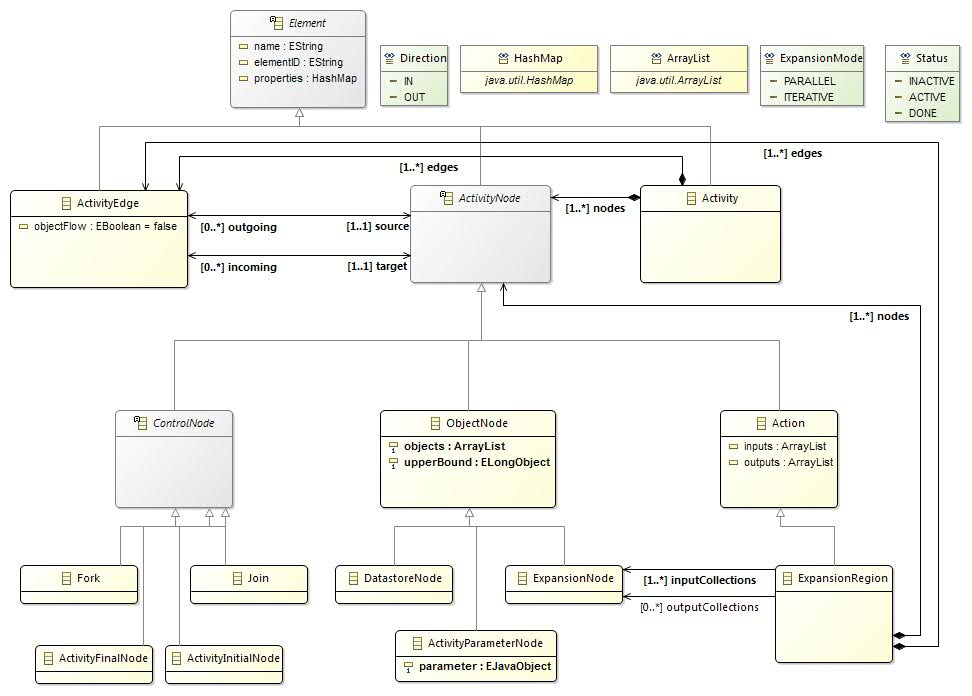
\includegraphics[width=38em]{./Figures/UML_Activity_mine_class_diagram}
		\rule{38em}{0.5pt}
	\caption[DSL Metamodel]{Metamodel of the DSL for provisioning and deployment of multi-cloud applications}
	\label{fig:Metamodel}
\end{figure}

\noindent 

\noindent Moreover, below is the list of the UML Activity Diagram constructs that we skipped with some explanations why we skipped them:

\begin{enumerate}
\item  ActivityGroup: generic construct to group nodes or edges, no need for it except ExpansionRegion which we use. ExpansionRegion is one of the subclasses of ActivityGroup.

\item  Pin: used when object is passed only between two actions, as a combination of data and control flows.

\item  CentralBufferNode: very similar to DatastoreNode, but can not connect directly to actions, acts as a storage place for other object nodes, so it is not needed.

\item  Merge and Decision nodes: see discussion above.

\item  FlowFinalNode: could be useful to stop parallel flows and avoid join nodes in some cases, but currently we consider it to be not very significant and have not. included it in the DSL

\item  ActivityPartition: subclass of ActivityGroup, often corresponds to organizational units in business model, not needed in the deployment plan.

\item  ParameterSet: a complete set of inputs and outputs to activities, may be used in scenarios with multiple activities and we work only with one activity.

\item  InterruptibleActivityRegion: used to handle exception events that we decided not to include.

\item  ExecutableNode: abstract class for nodes that may be executed, used as an attachment point for exception handlers in UML Activity Diagrams, so we do not include it.

\item  StructuredActivityNode: it is another abstraction of ActivityGroup, as we stated before we use only ExpansionRegion to group multiple similar actions and execute them sequentially or in parallel.

\item  SequenceNode: a node that can execute internal actions in sequence, we may use ExpansionRegion in such situations.

\item  LoopNode: we decided to avoid using loops.

\item  ConditionalNode: node that represents exclusive choice that we do not need.

\item  ExceptionHandler: see discussion above.
\end{enumerate}

\noindent To have even better understanding of the DSL, Figure \ref{fig:simplified} depicts simplified deployment plan of the storm cluster with one Supervisor node, using the described graphical notation of the language constructs.

\noindent The metamodel of our language is defined as a set of Java classes\footnote{ DSL for provisioning and deployment of multi-cloud applications, $  $https://github.com/SINTEF-9012/cloudml/tree/Maksym/deployer2/src/main/java/org/cloudml/deployer2/dsl}. In addition to that, we created an internal DSL to abstract low-level operations with language constructs. Internal DSLs (or embedded DSLs) are DSLs represented within the syntax of a general-purpose language - Java in our case \cite{fowler2010domain}. The usage of the internal DSL helps to reduce the number of possible errors during the creation of the deployment plan, and allows manipulations on the deployment plan. In addition, internal DSL could be used by the third party applications to adapt deployment plans. 

\begin{center}
	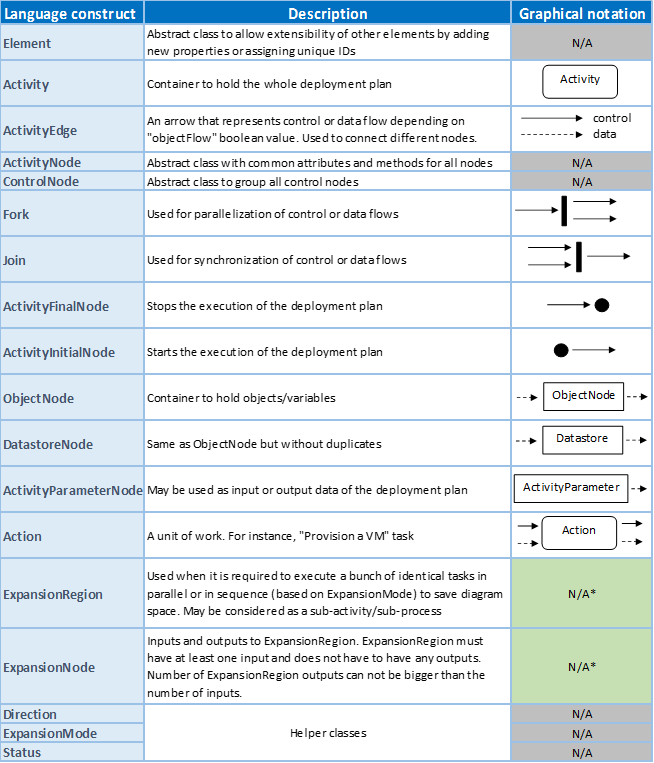
\includegraphics[width=38em]{./Figures/UML_table}
	\begin{table}[htbp]
    \caption{Description of the DSL Metamodel}
    \label{tab:2}
	\end{table}
\end{center} 

\begin{figure}[htbp]
	\centering
		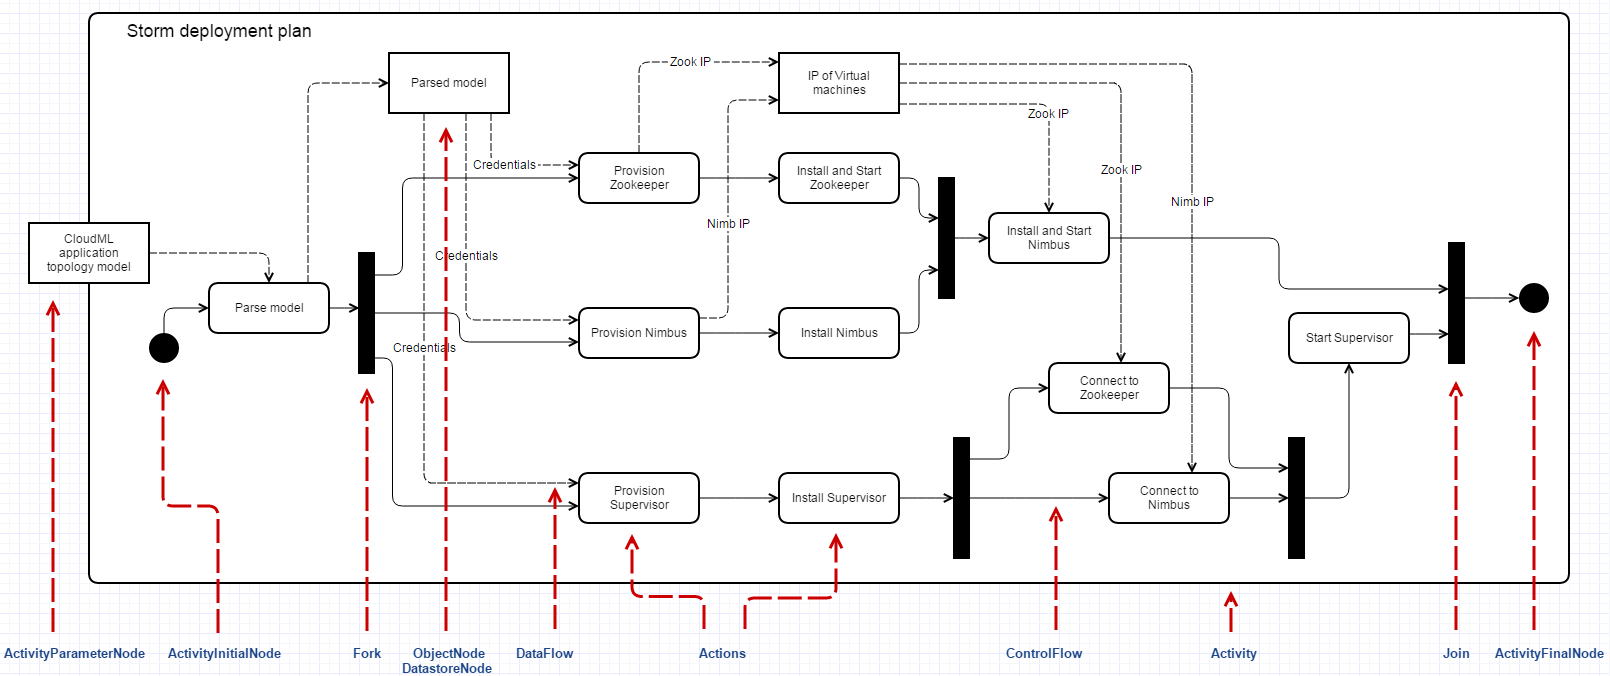
\includegraphics[width=38em]{./Figures/DSL_examplified}
		\rule{38em}{0.5pt}
	\caption[Storm Cluster Simplified Plan]{Simplified deployment plan of a storm cluster}
	\label{fig:simplified}
\end{figure}

%----------------------------------------------------------------------------------------
\subsection{Java Deployment Plan Builder as an Internal DSL}

\noindent To make things clearer, let us consider deployment DSL constructs in the space of our initial example - deployment of the storm cluster. The whole deployment plan for the storm application will be represented as an Activity and can be created with the help of the internal DSL as follows:

\begin{center}
	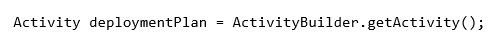
\includegraphics{./Figures/Get}
	\begin{lstlisting}[mathescape,caption={Deployment plan declaration},label={lst:3}]
	\end{lstlisting}
\end{center}

\noindent which will create an empty activity without any nodes or edges, so we can add nodes and edges to it. The deployment plan needs to start its executions at some point, so we start from the creation of the starting point:

\begin{center}
	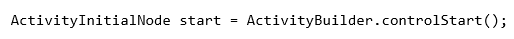
\includegraphics{./Figures/Start}
	\begin{lstlisting}[mathescape,caption={Activity initial node},label={lst:4}]
	\end{lstlisting}
\end{center}

\noindent which creates an initial node with one outgoing edge and adds this node and edge to the ``deploymentPlan'' that we created before. The first thing that has to be done during the deployment is the provisioning of virtual machines. We have three of them, so it is good to run provisioning in parallel, thus we have to create a fork node and three action nodes:

\begin{center}
	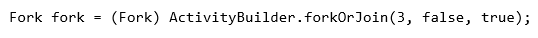
\includegraphics{./Figures/Fork}
	\begin{lstlisting}[mathescape,caption={Fork or Join node},label={lst:5}]
	\end{lstlisting}
\end{center} 

\noindent ``forkOrJoin'' method has three parameters: number of parallel edges, boolean to state if we are dealing with data or control flow, and boolean to decide if we want to create Fork or Join node. Fork node has one incoming and multiple outgoing edges and Join  the opposite: multiple incoming and one outgoing, other than that there is no difference between these two nodes. Both fork and join nodes may be dealing with only data flow or only control flow. The following situations are not allowed by the UML semantics: an incoming edge is a data edge and the outgoing edges are control edges - that is why we need second parameter. Moreover, the first parameter simply tells how many outgoing or incoming, data or control flow edges needs to be created. When fork with all edges is ready, we have to create three provisioning actions and connect them with Fork node, and also connect fork node with start node, because currently it is just a node that belongs to activity and not connected to anything. Actions:

\begin{center}
	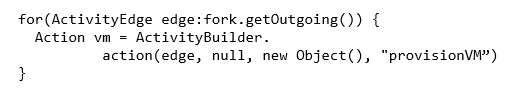
\includegraphics{./Figures/Action}
	\begin{lstlisting}[mathescape,caption={Action node},label={lst:6}]
	\end{lstlisting}
\end{center} 

\noindent ``action'' method has four parameters: incoming control edge, incoming data edge, incoming object and the name of the action. Every action must have an incoming control edge, it may also have incoming data edge (that is why we put null as a second parameter), it also may have input data and definitely some name. Regarding input data, if we think about real deployments every action will have some input: it may be credentials to the cloud provider, credentials to connect to specific VM, name of the command to invoke, shell script or anything else. In the code above, we iterate over outgoing control edges from the fork node and use them as incoming edges to every action, so action are already connected to the fork node. As we mentioned before, we also need to connect fork and start nodes:

\begin{center}
	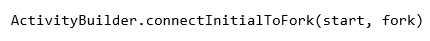
\includegraphics{./Figures/Connect}
	\begin{lstlisting}[mathescape,caption={Connecting two nodes},label={lst:7}]
	\end{lstlisting}
\end{center} 

\noindent This method obviously connects ActivityInitialNode with Fork node, and in addition it performs some more work with the deployment plan. Additional work includes validations that start and fork nodes are connected properly, for instance, if fork node had an incoming edge, then no need to create another edge for a start node. Basically, every method in the ActivityBuilder class that starts with a ``connect'' word performs similar kinds of validations.

\noindent 

\noindent Usually, after provisioning of virtual machines is done, IP addresses of these machines would be needed for further configuration. That is when data flow and object nodes come into play. In the scenario of storm deployment, IP address of Zookeeper VM is needed for configuration of Nimbus and Supervisor components, and IP address of Nimbus VM is needed for the configuration of Supervisor. We can save them all in one place for convenient retrieval. For this we have to create a Join node to synchronize data flows from ``provisionVM'' actions and then Object node to store IP addresses. An assumption here that all provisioning actions are gathered in one list:

\begin{center}
	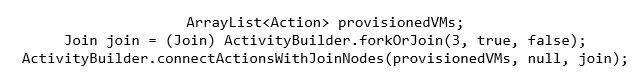
\includegraphics[width=38em]{./Figures/Join}
	\begin{lstlisting}[mathescape,caption={Join node},label={lst:8}]
	\end{lstlisting}
\end{center} 

\noindent Recalling parameters of the ``forkOrJoin'' method, the second parameter means that we are dealing with data flow, and the third - that we want to create a Join node, not Fork node. Then, ``connectActionsWithJoinNodes'' method has three parameters: an array of actions, Join node with control edges and Join node with data edges. In most cases the user would want to connect a set of actions with a Join node of the specific type (with control or data edges), so one parameter would be null, but in case both data and control flow from actions must be synchronized ~- it is possible to do that with this method. A caution for this method: number of actions must not be bigger than the number of incoming edges to Join node, ideally it should be the same. If it will be smaller - you shall remember that there are some edges left in the Join node that do not have any source node and you need to handle them later. What is left after previous calls - to create an Object node and connect it with Join node (Listing \ref{lst:9}). ``objectNode'' is one method to create different kinds of object nodes (Parameter, Datastore, Expansion, Object) with different possible configurations of edges (In, Out, InOut, NoEdges). The first parameter is object node name, second - node type, third - edges configuration.

\begin{center}
	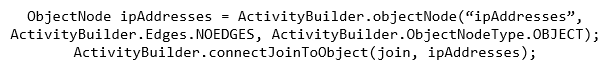
\includegraphics[width=38em]{./Figures/Object}
	\begin{lstlisting}[mathescape,caption={Object node},label={lst:9}]
	\end{lstlisting}
\end{center} 

\noindent Moreover, after creating object node we connect it to the Join node that was created before. One more thing, we did not mention yet how objects are passed between nodes. Currently we are creating a deployment plan, but IP addresses may be saved only after plan execution. So, assuming we have a provisioning action that has one output object with IP address of the provisioned virtual machine, and we have an Object node to store that IP, the process may look like this:

\begin{center}
	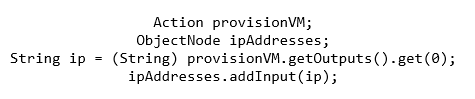
\includegraphics{./Figures/IP}
	\begin{lstlisting}[mathescape,caption={Adding data to the Object node},label={lst:10}]
	\end{lstlisting}
\end{center} 

\noindent So far we have shown how to create different kind of nodes and how to connect them. Concerning the storm example, we created a part of the deployment plan where all virtual machines are provisioned and their IP addresses are saved in one Object node for later retrieval. In a similar fashion we can create nodes and edges for all other installation and configuration commands and finish our deployment plan. Important note regarding ActivityBuilder class - for now it does not have any methods for manipulation on ExpansionRegion. Because we are working with CloudML and it does not have any constructs to group a number of tasks yet, we did not implement ExpansionRegion helper methods in the ActivityBuilder class, but it can be used on its own and added to the deployment plan like this:

\begin{center}
	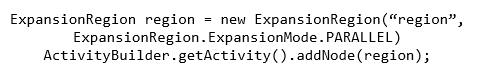
\includegraphics{./Figures/Region}
	\begin{lstlisting}[mathescape,caption={Expansion Region node},label={lst:11}]
	\end{lstlisting}
\end{center} 

\noindent After the generation of the deployment plan, it is important to check if we have not missed anything and everything is properly connected. For that we created a deployment plan validator (ActivityValidator.java class) which checks our model according to the following rules:

\noindent \begin{enumerate}
\item Check if all edges have source and target nodes. Edges can not point to nowhere or come from nowhere.

\item  Check if control edges do not have any kind of ObjectNode as source or target.

\item  Check if all nodes have incoming and outgoing edges to avoid control or data flows that do not lead to the final node. Exceptions here: ActivityFinalNode, ActivityInitialNode and ActivityParameterNode - all of them must have only one edge.

\item  Check if Action nodes have at least one incoming and at least one outgoing control edge because they must be triggered and lead to some other node

\item  Check if source nodes of incoming edges do not match with target nodes of outgoing edges of a given node to avoid cycles. Unfortunately, this rule does not check if there are bigger cycles in the deployment plan, like node number ten points back to node number one.

\item  Check if the activity has initial and final nodes to make sure it can be started and will be terminated eventually.

\item  Check if the activity has only one initial and only one final node to avoid ambiguities or conflicts during the deployment plan execution.
\end{enumerate}

%----------------------------------------------------------------------------------------
\section{Deployment Process} 

%----------------------------------------------------------------------------------------
In this section we explain in details how the deployment process is performed along with the usage of our DSL during the process execution.

\subsection{Introduction} 

\noindent A DSL by itself is useless unless it is used in conjunction with a deployment engine, so the next step is to integrate CloudML with our DSL to enable a transparent deployment process. The integration in this case means the transformation of the CloudML application topology model into the deployment plan - activity diagram with different nodes and edges, and then proper execution of such plan. Following an MDE approach, the transformation is defined at the metamodel level. This means that such an approach is generic and can be used to transform any CloudML model into a deployment plan as long as it conforms to the metamodel. A general idea of the transformation is depicted on Figure \ref{fig:high}.

\noindent 

\begin{figure}[htbp]
	\centering
		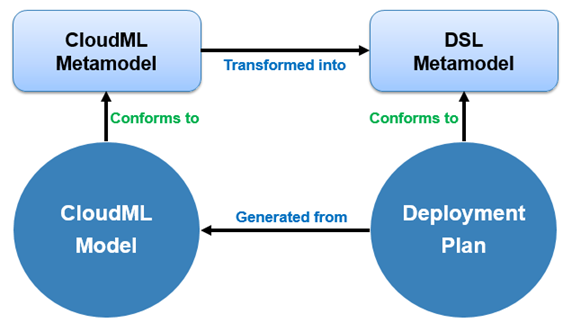
\includegraphics[width=32em]{./Figures/Transformation}
		\rule{38em}{0.5pt}
	\caption[High-level Transformation]{Models transformation (high-level)}
	\label{fig:high}
\end{figure}

\noindent 

\noindent The deployment plan shall represent every command that is executed during the deployment process and all dependencies between those commands to execute them in the proper order. The plan is generated according to the internal rules of the deployment engine (CloudML in our case) but generated sequence of commands might not suit specific needs of the user. For instance, default rules of the deployment engine may be to install every component on virtual machines and then configure them, but the requirement for some application component might be to perform some configuration (for example, set particular environment variables) and then execute an installation command. For the deployment specialist, in order to make a proper evaluation of the deployment plan (whether any changes are needed), it is important to see such plan in a graphical representation. After analyzing the plan he shall be able to execute it without any changes or rearrange the plan according to his needs. In case any changes to the plan were made, it is also important to be sure that the plan is still valid -- that it does not contain any structural errors. Finally, even after the validation the deployment plan can not be enacted immediately. To make actual deployment, the deployment engine has to create executable objects based on activity nodes and edges, a number of threads for parallel execution and then run them all in a proper order. The whole process is presented on Figure \ref{fig:details}:

\noindent 

\begin{figure}[htbp]
	\centering
		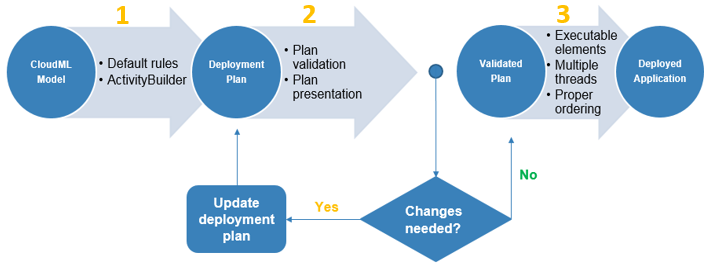
\includegraphics[width=38em]{./Figures/Details}
		\rule{38em}{0.5pt}
	\caption[Approach Details]{Approach details}
	\label{fig:details}
\end{figure}

\noindent 

\begin{figure}[htbp]
	\centering
		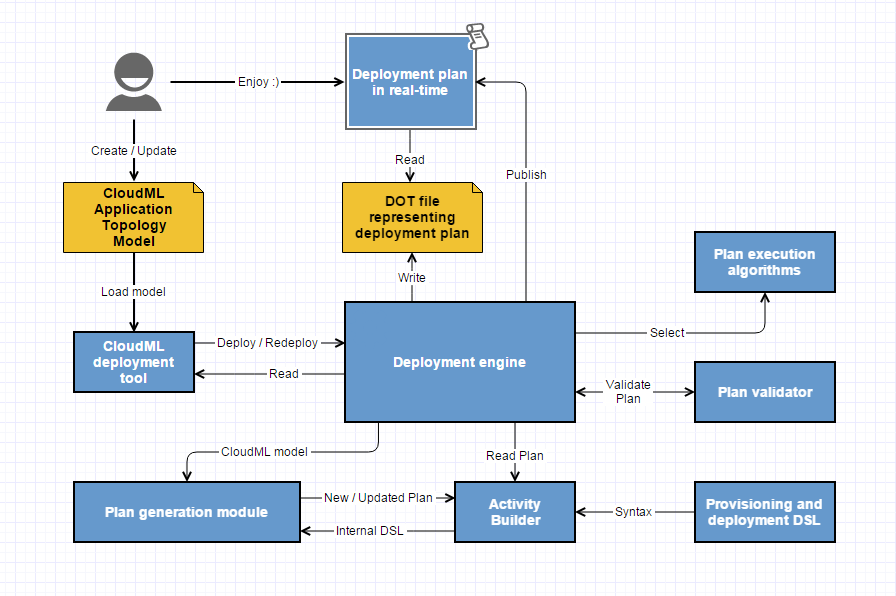
\includegraphics[width=38em]{./Figures/Architecture}
		\rule{38em}{0.5pt}
	\caption[Solution Architecture]{Solution architecture}
	\label{fig:architecture}
\end{figure}

\noindent 

\noindent Figure \ref{fig:architecture} depicts the overall architecture of the deployment system. The core element here is the deployment engine which orchestrates all other components. Referring to the deployment phases defined in the Figure \ref{fig:details}, during the first phase, the Deployment engine submits CloudML model to the Plan generation module. After that, according to the default rules and using the Internal DSL from the Activity Builder, the deployment plan is generated by the Plan generation module and saved in the Activity Builder. During the second deployment phase, the Deployment engine validates the plan through the Plan validator module and generates a DOT file (see Section \ref{subsec:presentation}) which can be used to visualize the deployment plan. Finally, during the third phase the Deployment engine executes the Deployment plan with selected algorithm and the execution process is displayed in real-time to the user.

%----------------------------------------------------------------------------------------

\subsection{Transformation of the Deployment Topology into Deployment Plan} 

\noindent The next step is to discuss each transformation in more details. First, we explain the transformation from the CloudML model to the Deployment Plan. Transformation in this case is based on a set of the default provisioning and deployment rules and on the generation of the Activity Diagram (deployment plan) nodes and edges with a help of our internal DSL, as discussed before. There are four default rules that are executed 

\begin{center}
	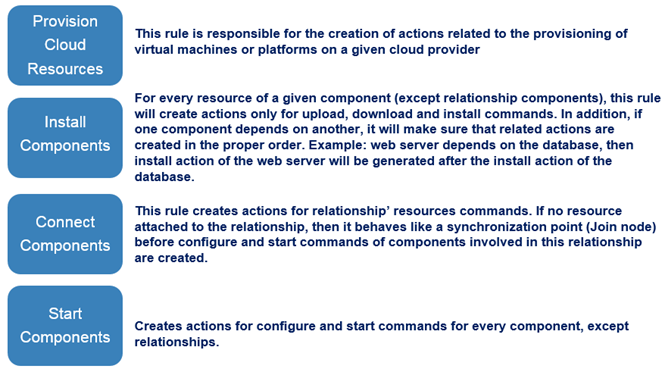
\includegraphics[width=38em]{./Figures/Rules}
	\begin{lstlisting}[mathescape,caption={Default rules of the CloudML deployment engine},label={lst:12}]
	\end{lstlisting}
\end{center}  

\noindent sequentially and they are explained on Listing \ref{lst:12}. These rules execute commands associated to CloudML components. In CloudML each component may have a resource attached to it and such resource may contain several commands like download, install, configure, start. Components may be databases, web servers, relationships.

\noindent During the execution of each rule, ActivityBuilder is used to create relevant components of the deployment plan. This is how the transformation from the CloudML model to the Deployment plan is done. Another interesting details is to understand how created actions are related to the real API calls to deploy the application. We can explain this with an example. For instance, let us take the declaration of the install command method from the CloudML:

\begin{center}
	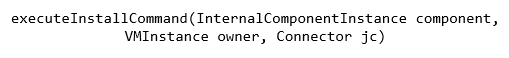
\includegraphics[width=38em]{./Figures/Install}
	\begin{lstlisting}[mathescape,caption={Install command declaration},label={lst:13}]
	\end{lstlisting}
\end{center}

\noindent We can not call this command during the creation of the deployment plan, but we have to know that exactly this command with such parameters must be called in the future. This can be accomplished by creating an Action with input objects that correspond to the input parameters of the executeInstallCommand and by setting the name of the action to ``executeInstallCommand''. This name can be used later to create a call to an actual method at run-time with the help of the Java reflection API\footnote{ The Java Reflection API, $  $https://docs.oracle.com/javase/tutorial/reflect/}. Assuming we have our input objects, we can create an action with multiple inputs like this:

\begin{center}
	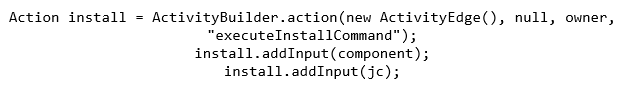
\includegraphics[width=38em]{./Figures/Inputs}
	\begin{lstlisting}[mathescape,caption={Passing data to actions},label={lst:14}]
	\end{lstlisting}
\end{center}

\noindent Apart from this detail, on Figures \ref{fig:provision}-\ref{fig:start_rule} we depict small algorithms to create a deployment plan in the context of the default deployment rules of the CloudML. During the execution of the Provision Cloud Resources rule (Figure \ref{fig:provision}) we have to create corresponding actions and nodes, but creation depends on the number of VMs. If we have several of them, then Fork node must be create and a Join node to gather data flows from all provisioning actions. Otherwise, if there was only one VM we could connect it directly to the Object node which stores IP addresses.

\noindent 

\begin{figure}[htbp]
	\centering
		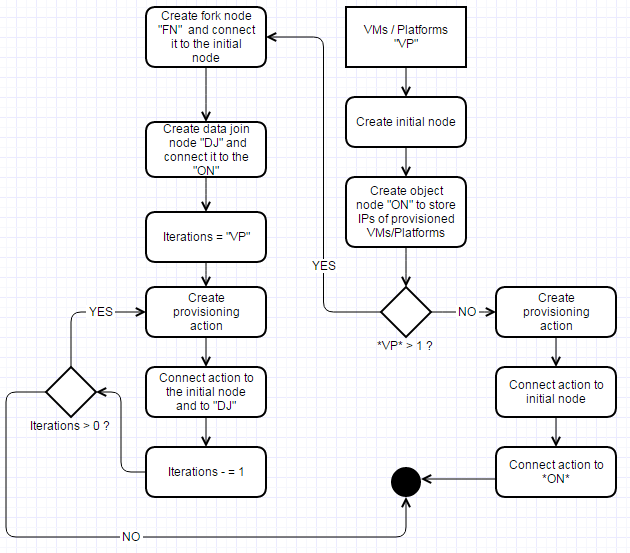
\includegraphics[width=38em]{./Figures/Provision_cloud_resources}
		\rule{38em}{0.5pt}
	\caption[Provisioning Rule]{Creation of the deployment plan during the execution of the Provision Cloud Resources rule}
	\label{fig:provision}
\end{figure}

\noindent 


\noindent 

\begin{figure}[htbp]
	\centering
		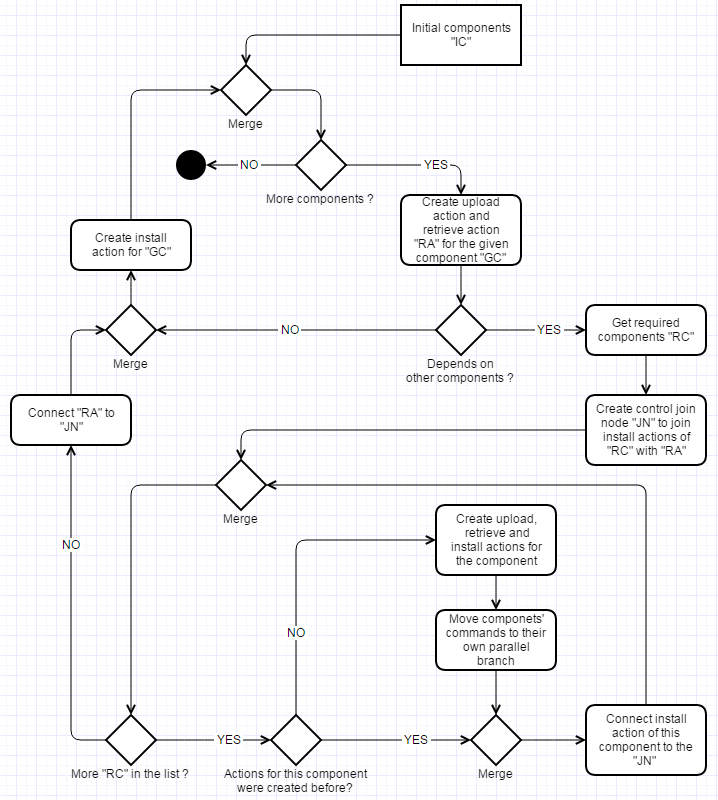
\includegraphics[width=38em]{./Figures/Install_components}
		\rule{38em}{0.5pt}
	\caption[Installation Rule]{Creation of the deployment plan during the execution of the Install Components rule}
	\label{fig:install_rule}
\end{figure}

\noindent

\noindent On Figure \ref{fig:install_rule} an algorithm to create components' install actions is showed. Imagine a servlet component which relies on the Tomcat server, which needs an SQL database to function properly. Assume SQL component was first in the list of components, then all installation actions for the SQL would be created. Then, second component is our servlet. The algorithm would detect that Tomcat must be installed, but before that -- SQL. Because SQL actions were already created, only actions for Tomcat will be generated, and only after that -- actions for the servlet component. 

\noindent 

\begin{figure}[htbp]
	\centering
		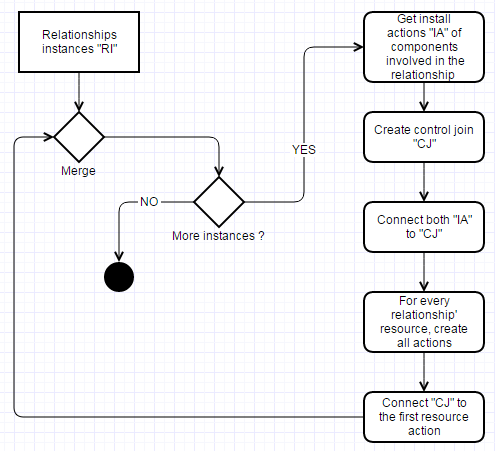
\includegraphics[width=38em]{./Figures/Connect_components}
		\rule{38em}{0.5pt}
	\caption[Connection Rule]{Creation of the deployment plan during the execution of the Connect Components rule}
	\label{fig:connect_rule}
\end{figure}

\noindent 

\noindent Figure \ref{fig:connect_rule} shows a simple algorithm which joins install actions of both components involved in the relationship. After that it creates actions that handle components' resources. If both involved components have attached resource, then additional Fork and Join nodes must be created to allow parallel execution of the resources actions.

\noindent 

\noindent Finally, the algorithm on Figure \ref{fig:start_rule} depicts the creation of configure and start actions. General rule is to connect the install action of the component to its configure action, and then configure action to the start action. In case a given component depends on another one, we create a Join node that synchronizes configure action of the current component with start action of the required component. After that Join node is connected to the start action. Finally, when all actions of all components are created, we join all deployment plan branches (usually each branch represents installation and configuration of one component) and create a Final node. That is when the transformation from the deployment topology to the deployment plan is completely finished. 

\noindent 

\begin{figure}[htbp]
	\centering
		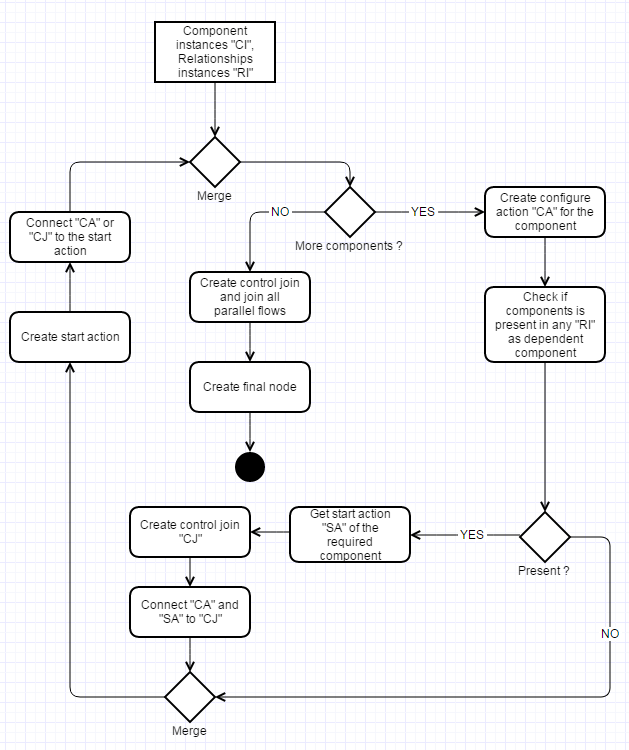
\includegraphics[width=38em]{./Figures/Start_components}
		\rule{38em}{0.5pt}
	\caption[Starting Rule]{Creation of the deployment plan during the execution of the Start Components rule}
	\label{fig:start_rule}
\end{figure}

%----------------------------------------------------------------------------------------

\subsection{Deployment Plan Validation and Presentation} 
\label{subsec:presentation}

\noindent The second step in our approach is the validation and presentation of the deployment plan. Validation is done according to the rules we defined before. After the validation is done, it is important to present the plan to the user. Ideally there would be some running web service that consumes our plan, displays it to the user and allows interactive manipulations. It would require a lot of time and work, so in the current implementation we went for rather a simplistic approach where DOT\footnote{ DOT language, $  $http://www.graphviz.org/pdf/dotguide.pdf} file is generated and presented to the user in the web page. It can also be represented with a help of many free online tools such as GraphvizFiddle\footnote{ GraphvizzFiddle tool, $  $http://stamm-wilbrandt.de/GraphvizFiddle/}. DOT language allows drawing directed graphs as hierarchies, so it nicely fits our needs as deployment process is a set of actions executed one after another. The syntax is quite simple and Listing \ref{lst:15} depicts a fragment of the DOT file and its representation on Figure \ref{fig:dot_image}:

\begin{center}
	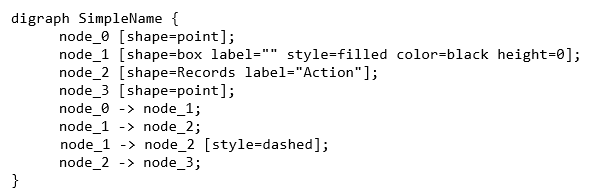
\includegraphics[width=38em]{./Figures/Dot}
	\begin{lstlisting}[mathescape,caption={Fragment of the DOT file},label={lst:15}]
	\end{lstlisting}
\end{center}

\begin{figure}[htbp]
	\centering
		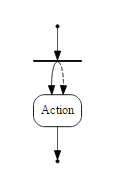
\includegraphics{./Figures/dot_image}
		\rule{38em}{0.5pt}
	\caption[DOT Image]{An image generated from the DOT file}
	\label{fig:dot_image}
\end{figure}

\noindent 

\noindent The whole syntax consists from nodes (node\_0 for instance) which can have different properties and edges that connect nodes (node\_0 -$>$ node\_1) and also may have some properties. To show something more complex, below are two deployment plans: first generated for the storm example and the second - for another application with a bit more complex CloudML model in terms of dependencies between components.  

\noindent 

\noindent On the Figure \ref{fig:storm_deployment}, which shows the storm deployment plan, a reader can observe a few consequent join nodes without any actions between them - this happens because every component is expected to have all set of commands by default: upload, download, install, configure, start. Moreover, if some component does not have configure and start commands for instance - such ``gap'' will be created. This is not an issue as it does not affect execution anyhow, and it may be improved in the future to have a cleaner representation of the plan. One more question that may arise - how can we know the IP of which machine is passed to ``configure:connection\_NameOfCommand'' commands as it is not written explicitly on the data edge? Relationships are components that involve cooperation between two components. The component where a specific command will be executed can retrieve its own IP, so we only need to get an IP of the ``partner''. Take a look at ``configure:connectionRetrieve nimbus-i'' action: ``nimbus-i'' part of the name indicates that this command will be executed on the ``nimbus (Maksym)'' virtual machine. So we need to get IP of the other component involved in the relationship. Before ``configure:connectionRetrieve nimbus-i'' action there is a join node that connect install commands of the zookeeper and nimbus components, so our ``partner'' here is zookeeper component. This means that data edges that lead to ``configure:connectionRetrieve nimbus-i'' and ``configure:connection - Configure nimbus-i'' are passing IP address of the ``zookeeper (Maksym)'' virtual machine.

\noindent 

\begin{figure}[htbp]
	\centering
		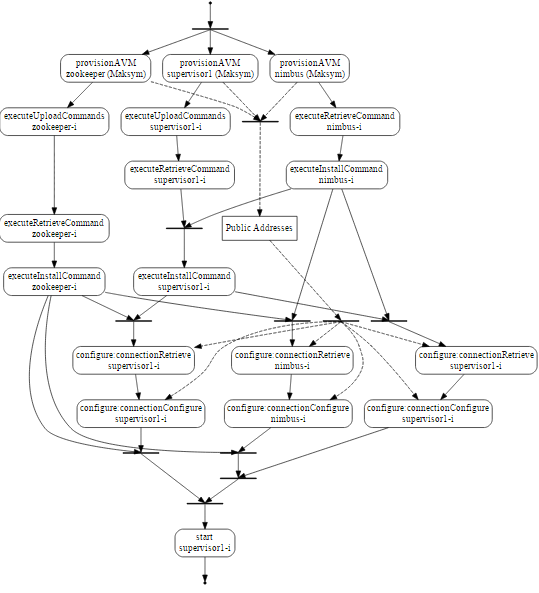
\includegraphics[width=38em]{./Figures/Storm_deployment_plan}
		\rule{38em}{0.5pt}
	\caption[Storm Deployment Plan]{Storm deployment plan}
	\label{fig:storm_deployment}
\end{figure}

\noindent 

\noindent The previous example was simple in a sense that each virtual machine had only one component installed on it and then we had six commands to configure relationships between each component. The deployment plan for another application that we tested is shown on Figure \ref{fig:hierarchy_plan}. It differs from the previous example in the number of components per virtual machine and dependencies between them. In this application we could talk about horizontal and vertical dependencies between components. By horizontal dependency we mean a connection between two independent components - like in the figure below sensApp1 component requires connection to the mongoDB1 component (it is a database). By vertical dependency we mean a situation when one component relies on the other, it just can not be installed without the first one being available - in our case sensApp1 (it is a servlet) needs jettySC1 component (servlet engine) to be installed, the same as sensAppAdmin1 component needs jettySC2 component.

\noindent 

\begin{figure}[htbp]
	\centering
		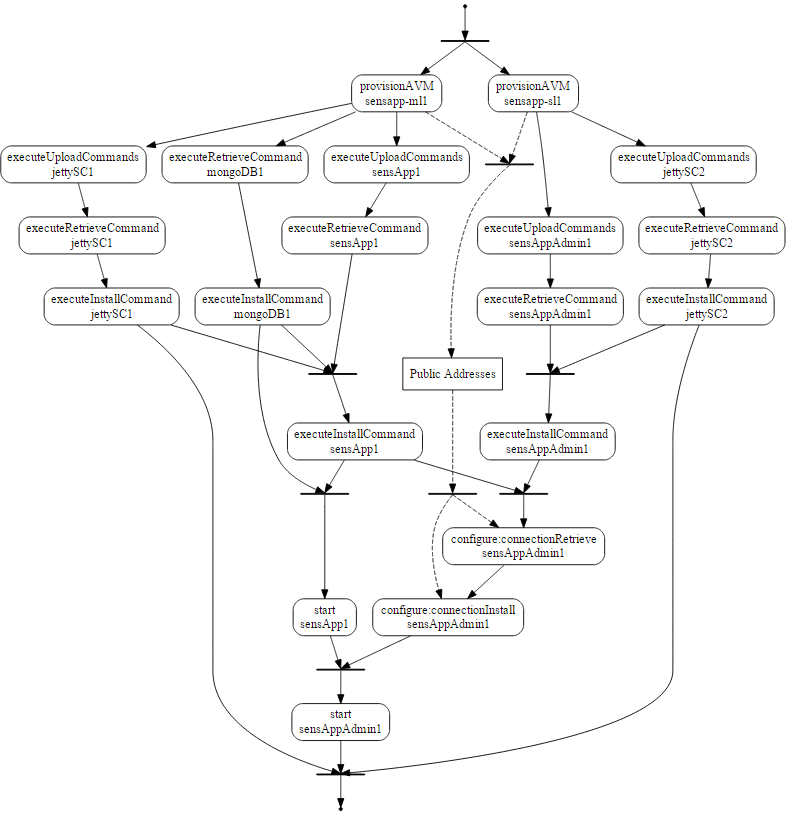
\includegraphics[width=38em]{./Figures/Sensapp_noSaas}
		\rule{38em}{0.5pt}
	\caption[Multi-level Hierarchy Plan]{Deployment plan of the application with multi-level dependency hierarchy}
	\label{fig:hierarchy_plan}
\end{figure}

\noindent 

\noindent To sum up, both examples presented before expose enough details about the deployment and provisioning commands and their ordering, so that the application developer can make a proper decision if the deployment process will be successful or some more adjustments to the plan are needed. In case the application owner decides to adjust the generated plan, he can do that with the help of the internal DSL which was described previously, so we will not go into details how to do it again.

%----------------------------------------------------------------------------------------

\subsection{Deployment Plan Enactment}

\noindent The next phase is the actual deployment of the application. Having the deployment plan generated and validated, the deployment engine has to traverse the graph in the proper order (taking into account parallelization and synchronization points) and execute each task. The execution of every task was covered before -- it is done with the help of Java Reflection API. As for parallelization and synchronization of separate graph branches, we use Java Fork/Join Framework\footnote{ Java Fork/Join framework: https://docs.oracle.com/javase/tutorial/essential/concurrency/forkjoin.html} which allows to start multiple threads asynchronously and join them later. 

\noindent The most difficult part of the plan execution is to actually make sure that every node and edge is visited and visited in a proper order. During the development of the prototype we actually came up with two approaches to traverse the graph. The first approach was inspired by the parallel breadth-first search algorithms which are often used to traverse graphs \cite{akeila2010object}. The idea here is to mark every node and edge with a number (``level'') and then execute nodes and edges of the same level in parallel (using the Fork/Join framework in our case). The leveling of node and edges is depicted on Figure \ref{fig:levels}.

\noindent 

\begin{figure}[htbp]
	\centering
		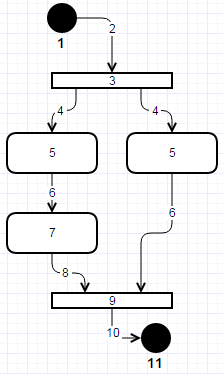
\includegraphics[height=18em]{./Figures/Parallel}
		\rule{38em}{0.5pt}
	\caption[Parallel Algorithm]{Assigning levels to the nodes and edges of the graph}
	\label{fig:levels}
\end{figure}

\noindent 

\noindent It is important to mention that levels do not represent the shortest distance from the source node, but rather the longest distance due to synchronization points. The limitation of such approach is that we achieve parallelism, but not concurrency -- distinct graph branches are not independent. In other words, executing tasks by levels is the same as having Fork and Join nodes for every set of parallel tasks . Thus, this approach is definitely faster than sequential execution of tasks, but not optimal.

\noindent To overcome this limitation, we developed another approach where each parallel branch can be executed in total independence from other branches as shown on Figure \ref{fig:concurrent}, thus achieving concurrency. In this approach, the deployment engine creates a number of threads whenever the it enters Fork node (explicit fork) or Action node with multiple outgoing edges (implicit fork), and joins multiple threads whenever it reaches Join node (explicit join) or Action node with multiple incoming edges (implicit join). Examples of the implicit fork and join are shown on Figure \ref{fig:implicit}. We do not cover many details of both approaches not to overload the reader with technical nuances, the source code is available for curious readers. 

\noindent 

\begin{figure}[htbp]
	\centering
		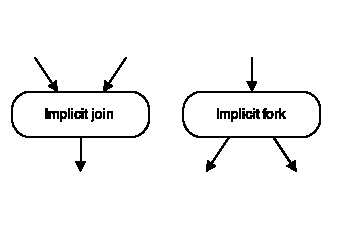
\includegraphics{./Figures/Implicit}
		\rule{38em}{0.5pt}
	\caption[Implicit Fork and Join]{Examples of the implicit fork and join}
	\label{fig:implicit}
\end{figure}

\noindent 

\begin{figure}[htbp]
	\centering
		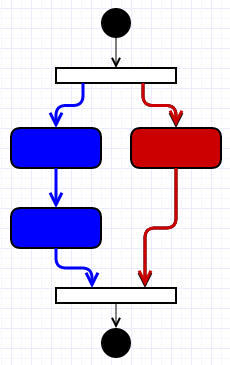
\includegraphics[height=18em]{./Figures/Concurrent}
		\rule{38em}{0.5pt}
	\caption[Concurrent Algorithm]{Execution concurrency: blue and red branches are independent threads}
	\label{fig:concurrent}
\end{figure}

\noindent

\noindent At the moment of writing, the second approach is operational but not yet fully stable - once in a while a deadlock may occur (5-10\% of the time). This will be fixed by the end of the internship. Nevertheless, it proved to be very useful during the development, testing and for the deployment of small applications. In the future, both approaches may be combined to have a robust concurrent deployment algorithm.

\noindent Another important development which resulted from the usage of the models@run-time pattern and from the graphical representation of the deployment plan is that our deployment plan is also a model@run-time. Each node and edge may be in one of the three states: Inactive, Active and Done. Before the graph traversal starts, all nodes and edges are in the state Inactive. Whenever the deployment engine enters some node or edge, it changes the state of that node or edge to Active and then to Done, when it exits that node or edge. All these state changes are reflected in the DOT file. To show this behavior in real time, we created a web page that displays the deployment process in real time. An example of the deployment process is shown on Figure \ref{fig:realtime}.

\noindent Last, but not least, is the description of the continuous deployment process. As we stated before, CloudML has a diff engine which calculates the differences between the old and a new application topology models. With regard to deployment plans, we could follow the same approach -- generate a deployment plan for the new model and then calculate the differences between the old and new plans to create an adaptation plan. Instead, we follow more efficient approach: the plan generation module takes as input new components of the application topology plan and removed components in comparison with the old application topology model. After that, based on the input components, an adaptation plan is generated. By following this approach we eliminate the need to create another diff engine just for the deployment plans by reusing existing algorithms for the plan generation. While generating an adaptation plan, the old deployment plan stays in memory to access important information from the previous deployments, such as IPs of provisioned virtual machines. Thus, the generation of the adaptation plan is based not only on the input components described above, but also on already executed actions. For instance, during the creation of the relationship actions, if require component was installed and started before, it will not be shown again in the adaptation plan. An example of the adaptation plan is shown on Figure \ref{fig:adaptation} -- it is generated after changing the application topology model of the storm cluster from having one supervisor node to two.

\noindent 

\begin{figure}[htbp]
	\centering
		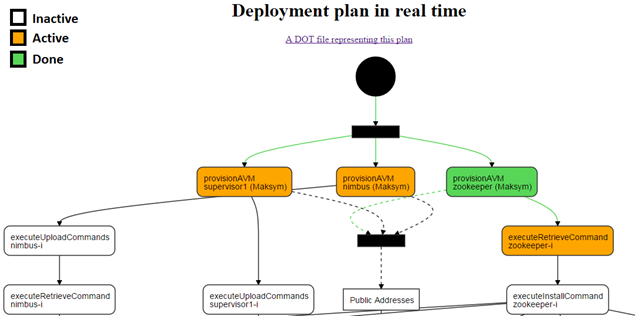
\includegraphics[width=38em]{./Figures/Realtime}
		\rule{38em}{0.5pt}
	\caption[Real-time Deployment]{Deployment process in real time}
	\label{fig:realtime}
\end{figure}

\begin{figure}[htbp]
	\centering
		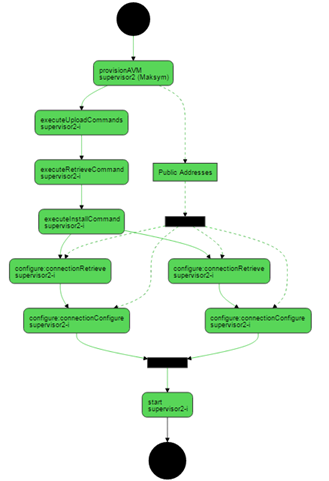
\includegraphics{./Figures/Adaptation}
		\rule{38em}{0.5pt}
	\caption[Adaptation Plan]{Adaptation plan of the storm cluster}
	\label{fig:adaptation}
\end{figure}


\noindent To conclude, the whole process of the deployment plan generation and execution is very complex. While we present a prototype, still a lot has to be done to generate proper plans from different application topologies, to generate proper adaptation plans in various continuous deployment scenarios and to have stable, yet fast, deployment execution algorithms. 



